\section{Prefetcher Enhancements}
\label{Enhancements}

\begin{figure}
  \begin{center}
  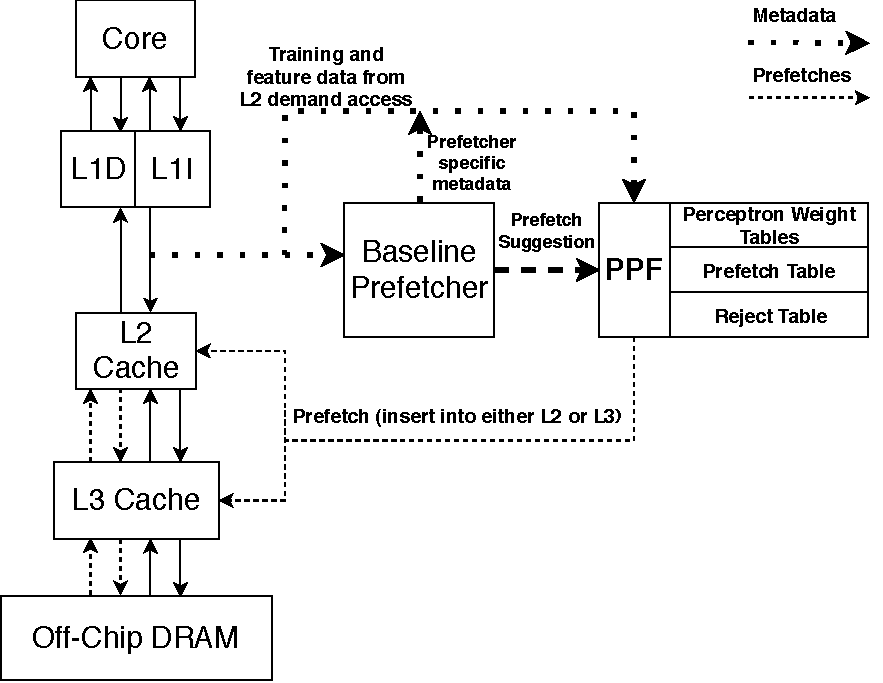
\includegraphics[width=8cm]{PPF_Hierarchy}
  \caption{PPF Architecture in the Memory Hierarchy}
  \label{fig:PPF_Hierarchy}
  \end{center}
\end{figure}

It can be beneficial to allow a prefetcher like SPP to speculate as 
deeply as possible. Often, some useful prefetches are generated long 
after the confidence of the prefetcher has fallen below the point at 
which performance degrades due to the increase of inaccurate prefetches.  
In order to allow deep speculation in the prefetcher, however, inaccurate
prefetches must be filtered out.  We propose to leverage
perceptron-based learning as a mechanism to differentiate between
potentially useful deeply speculated prefetches and likely not-useful
ones. The Perceptron based Prefetch Filter (PPF) is placed between the
prefetcher and the prefetch insertion queue, as illustrated in
Figure~\ref{fig:PPF_Hierarchy}, to prevent not-useful prefetches from
polluting the higher levels of the memory hierarchy.
Perceptron filter considers a number of features corresponding to a
prefetch, such as speculation depth, page address and offset, and uses
this information as the inputs to our perceptron-based filter in order
to predict the usefulness of a prefetch.  

\subsection{Changes made to SPP}
\label{Enhancements-SPP}
To modify the SPP design to suit our scheme, the following changes
were made:

\noindent \textbf{Adjusting Aggressiveness Level:}
This was done by tuning down the internal throttling mechanism to the 
extreme values to allow all the prefetches to pass through. As a 
consequence, the internal confidence mechanism was no longer used
to make prefetch or fill-level decisions.

\noindent \textbf{Adding Prefetch and Reject Filters:}
In our proposed approach, we need to reindex the perceptron tables (explained in
section XX\%) for training when the feedback from the prefetch is available.
To do that, we added two 1024-entry filters which would hold the data required to index
these tables. Depending on the decision of the perceptron (prefetch vs reject), the
data is stored in the respective tables.

\noindent \textbf{Exporting data between SPP and Perceptron:}
Perceptron learning uses the metadata associated with a prefetch suggestion as the
perceptron 'features'. Some of the features we developed use information derived 
directly from program execution. Beyond that, SPP also conveys some useful 
information like lookahead depth, signature, and the confidence counter to the 
perceptron filter.

\subsection{The Perceptron Filter}
\label{Enhancements-PPF}

\begin{figure}[ht]
  \begin{center}
  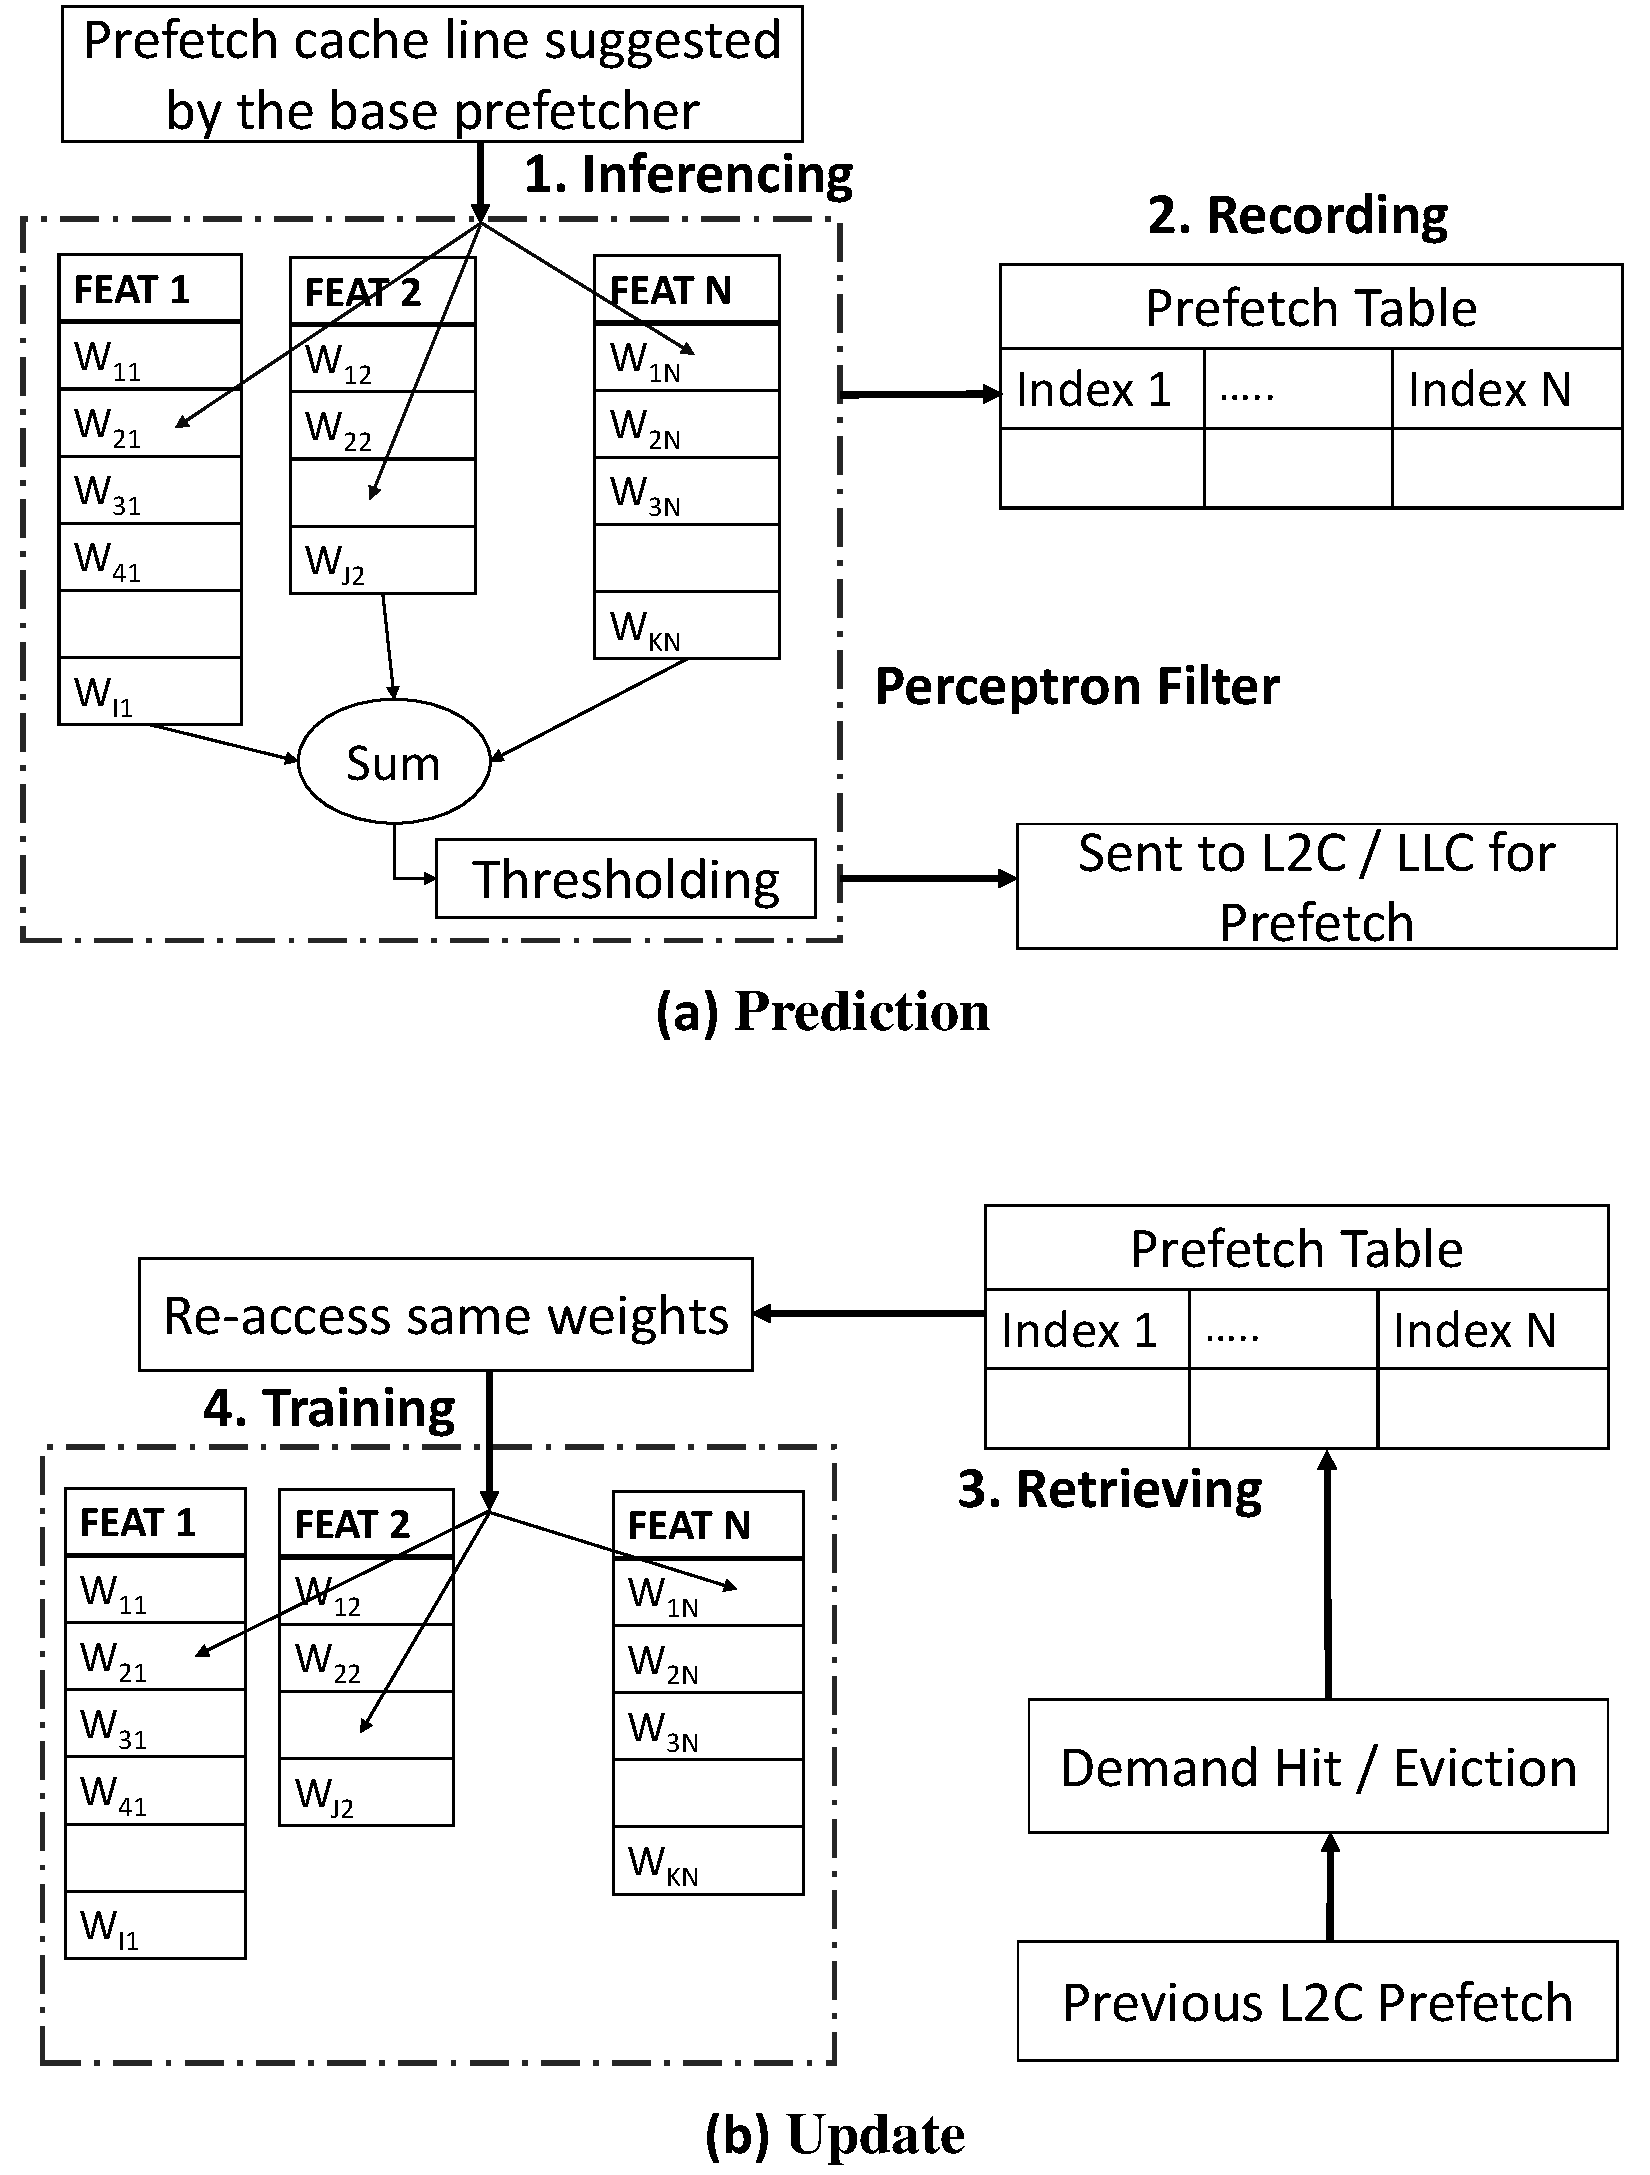
\includegraphics[width=\columnwidth]{Datapath_Separate}
  \caption{PPF Data Path and Operation}
  \label{fig:PPF_Datapath}
  \end{center}
\end{figure}

Figure~\ref{fig:PPF_Datapath} shows the microarchitecture of PPF, as
well as the steps required to filter out not-useful prefetches. The
perceptron filter is organized as a set of tables, where each entry in
the tables holds a \textit{weight}. Each table is indexed using a 
different number of bits from the corresponding feature. Each
weight is a 5-bit saturating counter ranging from -16 to +15. 

\noindent \textbf{Inferencing and Data Recording:}
SPP is triggered on every demand access to the L2 Cache. The suggested 
prefetch candidates from SPP are fed to the perceptron filter to determine 
their usefulness and fill-level. This is done by thresholding the perceptron 
dot-product sum against two different values: $\tau_{hi}$ and $\tau_{lo}$.
Depending on the outcome of the perceptron, the feature values are recorded
in one of the two filters introduced above.

\noindent \textbf{Data Retrieval and Training:}
PPF training is triggered whenever a prefetched block leads to a demand hit
or a cache eviction. A valid entry in one of the tables means that the current
memory access was a prefetch candidate in the past. The retreived feature values 
are used to index the tables of weights. A uniform perceptron update rule
is followed. If the prediction was correct (prefetched cache line leading to a 
demand hit) and the perceptron sum lies within a predefined threshold, weights are 
updated in the correct direction. If the prediction was incorrect (prefetched cache 
line getting evicted without getting used or a prefetch reject leading to demand 
access), the weights are updated in the opposite direction.

\textit {Note: More details about PPF working and implementation can be found 
in the paper Perceptron-based Prefetch Filtering.}
\textcolor{blue}{Is it okay to allude to the PPF paper? Will it be possible to cite it?}

\subsection{Other Optimizations}
\label{Enhancements-Misc}

\noindent \textbf{Resource Division Across Pages:}
For prefetch friendly applications, an aggressive lookahead prefetcher can go really
deep down the speculation path. This takes up valuable resources in the system's Prefetch 
Queue (PQ) hence blocking any prefetch attempts from subsequent pages, leading to a timing
disparity bewteen pages interleaved across demand accesses. To avoid that, our prefetcher 
maintains a count of distinct pages being accessed in last-8 demand accesses and divides the
PQ resources across those many pages by limiting the maximum number of prefetches in a given 
page.
